\section{Latar Belakang}

Pemesanan hotel yang dibatalkan, terutama menjelang tanggal kedatangan,
meninggalkan kamar kosong yang sulit dijual kembali. Jika pembatalan dapat
diperkirakan sejak awal, hotel dapat mengambil langkah pencegahan, misalnya
meminta deposit atau menghubungi tamu lebih awal. Tugas ini membangun model
klasifikasi biner untuk memprediksi apakah sebuah pemesanan akan dibatalkan
(\texttt{is\_canceled} $=1$) atau tidak (\texttt{is\_canceled} $=0$) berdasarkan
data pemesanan~\cite{asisten2026spek}.

Kedua jenis kesalahan prediksi berdampak berbeda bagi hotel. \textit{False
negative} terjadi ketika pemesanan yang akhirnya dibatalkan diprediksi tidak
batal. Hotel tidak mengambil langkah apa pun, dan kamar tersebut berisiko kosong
setelah pembatalan terjadi. \textit{False positive} terjadi ketika pemesanan yang
sebenarnya datang diprediksi batal. Jika hotel menanggapinya dengan menjual kamar
yang sama ke tamu lain (\textit{overbooking}), tamu yang datang bisa tidak
mendapat kamar. Jika hotel menanggapinya dengan meminta deposit atau menghubungi
tamu, tamu yang sebenarnya akan datang ikut terbebani.

\textit{Dataset} ini tidak memuat biaya kedua jenis kesalahan tersebut sehingga
laporan ini tidak memberi bobot yang berbeda pada keduanya. Model dievaluasi
dengan \textit{macro F1-score} (Subbab~\ref{sec:distribusi-kelas}), yang
memperhitungkan kesalahan pada kedua kelas secara seimbang. Jika hotel mengetahui
kerugian masing-masing kesalahan, ambang keputusan model dapat digeser untuk
mengurangi jenis kesalahan yang lebih mahal.

\section{\textit{Dataset}}

\textit{Dataset} terdiri atas \texttt{data/train.csv} yang berlabel dan
\texttt{data/test.csv} yang tidak berlabel. Prediksi untuk data uji disimpan
dengan format \texttt{data/sample\_submission.csv}, yaitu kolom \texttt{id} dan
\texttt{is\_canceled}.

\begin{table}[H]
	\centering
	\caption{Ukuran \textit{dataset}}
	\label{tab:ukuran}
	\begin{tabular}{l r r}
		\toprule
		\textbf{Berkas} & \textbf{Baris} & \textbf{Kolom} \\
		\midrule
		\texttt{train.csv} & 27.373 & 19 (17 fitur, \texttt{id}, \texttt{is\_canceled}) \\
		\texttt{test.csv}  & 6.844  & 18 (17 fitur, \texttt{id}) \\
		\bottomrule
	\end{tabular}
\end{table}

\begin{table}[H]
	\centering
	\caption{Atribut \textit{dataset}}
	\label{tab:atribut}
	\small
	\begin{tabular}{l l p{6cm}}
		\toprule
		\textbf{Atribut} & \textbf{Tipe} & \textbf{Keterangan} \\
		\midrule
		\texttt{num\_adults}, \texttt{num\_children} & numerik & Jumlah tamu dewasa dan anak \\
		\texttt{weekend\_nights}, \texttt{weekday\_nights} & numerik & Jumlah malam akhir pekan dan hari kerja \\
		\texttt{meal\_package} & kategorikal & Room Only, Breakfast, Half Board, Full Board \\
		\texttt{needs\_parking} & biner & Tamu membutuhkan tempat parkir \\
		\texttt{room\_category} & kategorikal & Type A-G \\
		\texttt{days\_before\_arrival} & numerik & Selisih hari antara pemesanan dan kedatangan (\textit{lead time}) \\
		\texttt{arrival\_year/month/day} & numerik & Tanggal kedatangan (2023-2024) \\
		\texttt{booking\_channel} & kategorikal & Online Travel Agent, Offline Agent, Corporate, Complimentary, Airline \\
		\texttt{is\_returning\_guest} & biner & Tamu pernah menginap sebelumnya \\
		\texttt{prior\_cancellations} & numerik & Jumlah pembatalan sebelumnya \\
		\texttt{prior\_completed\_bookings} & numerik & Jumlah pemesanan sebelumnya yang tidak dibatalkan \\
		\texttt{nightly\_rate\_idr} & numerik & Harga kamar per malam (rupiah) \\
		\texttt{special\_requests} & numerik & Jumlah permintaan khusus \\
		\midrule
		\texttt{is\_canceled} & biner & Target: 1 jika pemesanan dibatalkan \\
		\bottomrule
	\end{tabular}
\end{table}

\section{Pemahaman Data}

Analisis eksploratif dibuat dengan fungsi di \texttt{src/eda.py} dan dijalankan
pada bagian \textit{Data Understanding} di \texttt{src/main.ipynb}.

\subsection{Distribusi Kelas}
\label{sec:distribusi-kelas}

Dari 27.373 baris data latih, 18.404 baris (67,2\%) tidak batal dan 8.969 baris
(32,8\%) batal (Gambar~\ref{fig:target}). Perbandingan kedua kelas sekitar 2:1.
Karena itu, model dievaluasi dengan \textit{macro F1-score} agar kinerja pada kelas
batal yang lebih sedikit berbobot sama dengan kelas tidak batal. \textit{Macro
F1-score} adalah rata-rata F1 kedua kelas.

\begin{figure}[H]
	\centering
	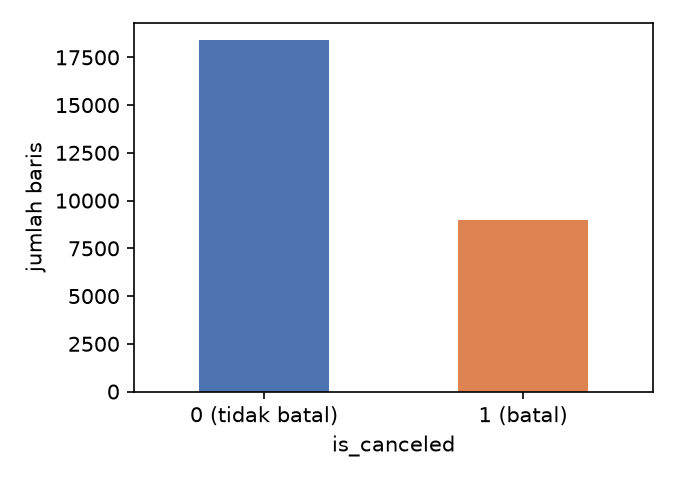
\includegraphics[width=0.55\textwidth]{target_distribution}
	\caption{Distribusi kelas \texttt{is\_canceled} pada data latih}
	\label{fig:target}
\end{figure}

\subsection{Nilai Hilang dan Duplikat}

Delapan atribut memiliki nilai hilang dengan proporsi yang hampir sama pada data
latih dan data uji (Tabel~\ref{tab:missing}). Imputasi yang di-\textit{fit} pada
data latih pun dapat diterapkan langsung ke data uji. Data latih memuat 66 baris
duplikat (seluruh fitur identik), data uji memuat 3 baris, dan gabungan keduanya
memuat 109 baris.

\begin{table}[H]
	\centering
	\caption{Persentase nilai hilang per atribut}
	\label{tab:missing}
	\begin{tabular}{l r r}
		\toprule
		\textbf{Atribut} & \textbf{Latih (\%)} & \textbf{Uji (\%)} \\
		\midrule
		\texttt{num\_children}        & 11,09 & 10,91 \\
		\texttt{special\_requests}    & 9,13  & 8,66 \\
		\texttt{nightly\_rate\_idr}   & 7,45  & 7,89 \\
		\texttt{meal\_package}        & 6,43  & 6,46 \\
		\texttt{days\_before\_arrival}& 4,10  & 4,24 \\
		\texttt{needs\_parking}       & 3,95  & 3,61 \\
		\texttt{room\_category}       & 3,66  & 3,54 \\
		\texttt{num\_adults}          & 2,96  & 2,63 \\
		\bottomrule
	\end{tabular}
\end{table}

\subsection{Sebaran Fitur dan Pencilan}

Sebagian besar fitur numerik menceng ke kanan. Median
\texttt{days\_before\_arrival} adalah 58 hari dengan maksimum 448 hari. Median
\texttt{nightly\_rate\_idr} adalah Rp1.644.000 dengan maksimum Rp9.165.000, dan
beberapa baris memiliki harga Rp0. Hampir semua nilai
\texttt{prior\_cancellations} dan \texttt{prior\_completed\_bookings} adalah 0.
Distribusi kategori juga timpang: Type B mencakup 75\% nilai
\texttt{room\_category}, Full Board hanya muncul empat kali pada
\texttt{meal\_package}, dan Airline hanya muncul 88 kali pada
\texttt{booking\_channel}.

\subsection{Korelasi dengan Target}

Gambar~\ref{fig:korelasi} menunjukkan korelasi Pearson antara setiap fitur numerik
dan target. Korelasi positif terbesar dimiliki \texttt{days\_before\_arrival}
(0,44): pemesanan yang dibuat jauh hari lebih sering dibatalkan. Korelasi negatif
terbesar dimiliki \texttt{special\_requests} ($-0{,}26$): tamu yang mengajukan
permintaan khusus lebih jarang membatalkan pemesanan. \texttt{arrival\_year} (0,18)
dan \texttt{nightly\_rate\_idr} (0,13) juga berkorelasi positif dengan pembatalan.

\begin{figure}[H]
	\centering
	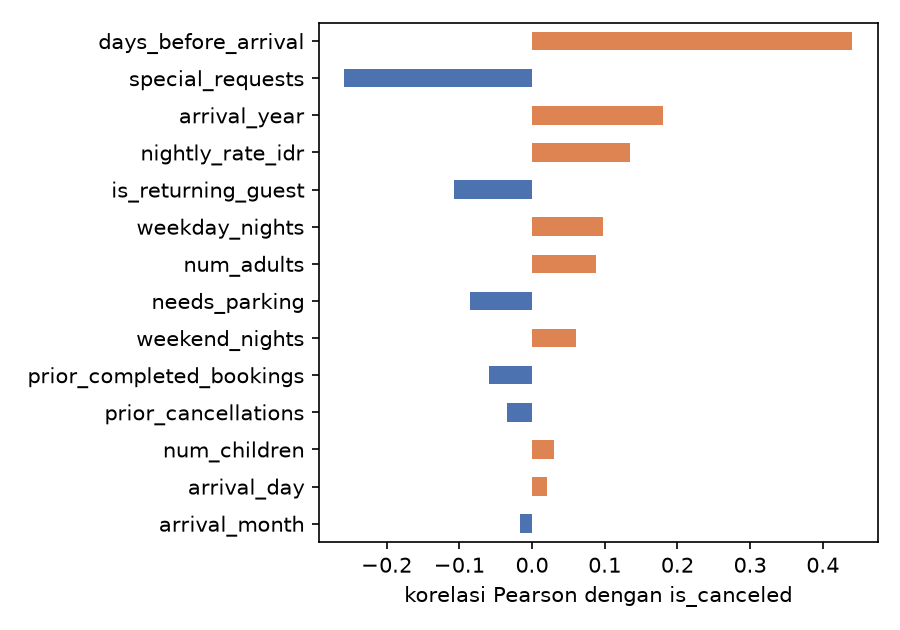
\includegraphics[width=0.75\textwidth]{correlation}
	\caption{Korelasi fitur numerik dengan \texttt{is\_canceled}}
	\label{fig:korelasi}
\end{figure}

\subsection{Rasio Pembatalan per Kategori}

Gambar~\ref{fig:target-rate} menunjukkan rasio pembatalan untuk setiap nilai
\texttt{booking\_channel}, \texttt{meal\_package}, \texttt{room\_category}, dan
\texttt{arrival\_month}. Gambar ini dibuat dengan fungsi \texttt{target\_rate} di
\texttt{src/eda.py}. Garis putus-putus menandai rasio pembatalan seluruh data
latih (32,8\%).

\begin{figure}[H]
	\centering
	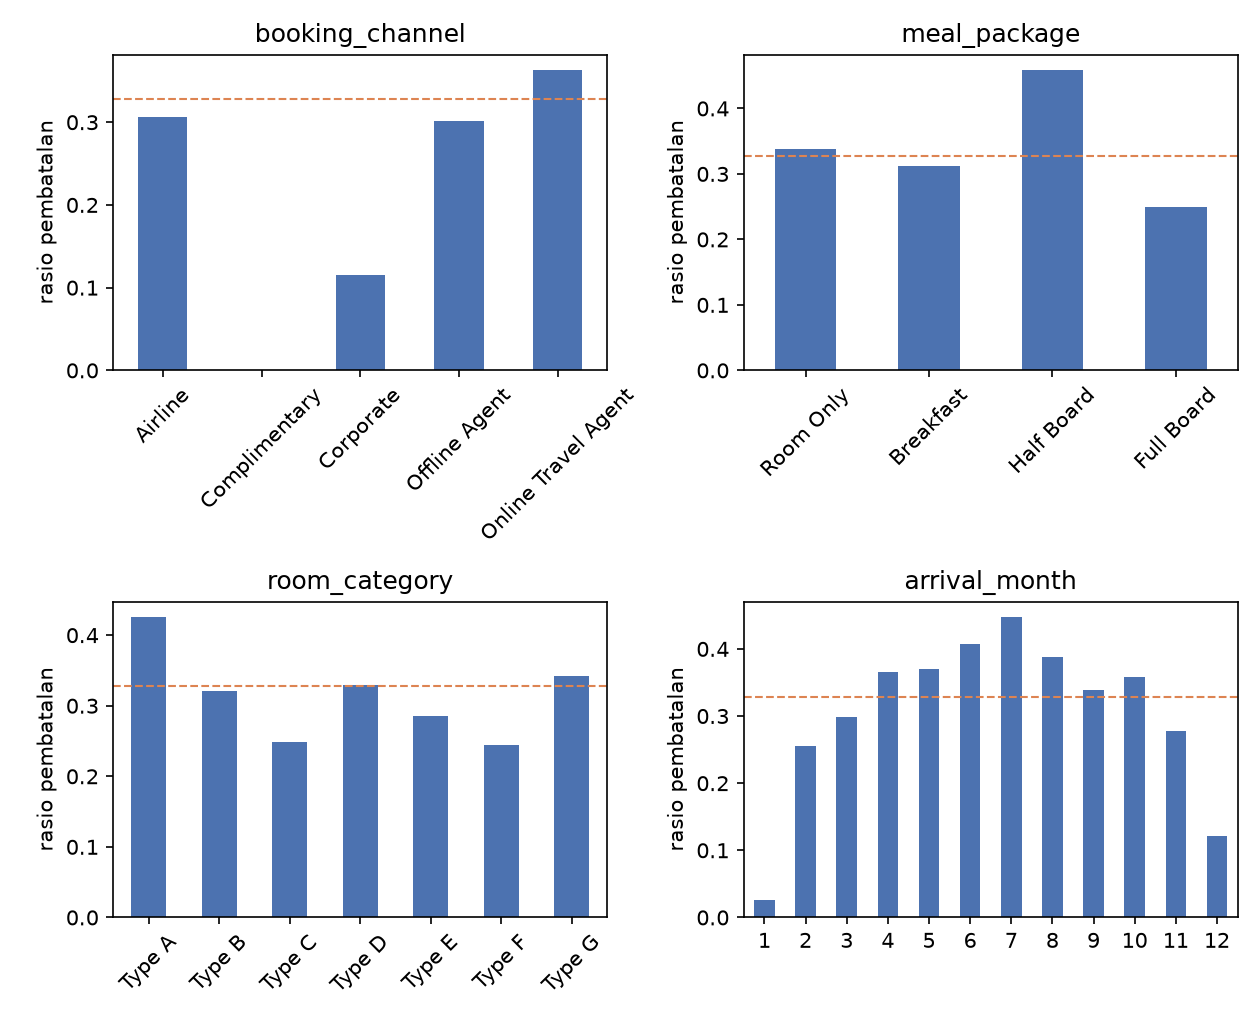
\includegraphics[width=0.95\textwidth]{target_rate}
	\caption{Rasio pembatalan per kategori pada data latih}
	\label{fig:target-rate}
\end{figure}

Perbedaan terbesar terlihat pada \texttt{booking\_channel}. Online Travel Agent,
kanal dengan 17.511 pemesanan, memiliki rasio pembatalan 36,4\%, sedangkan
Offline Agent memiliki rasio 30,2\%. Rasio pada Corporate hanya 11,5\%, dan tidak
satu pun dari 301 pemesanan Complimentary dibatalkan. Airline memiliki rasio
30,7\%, tetapi hanya berisi 88 pemesanan.

Pada \texttt{meal\_package}, Half Board memiliki rasio pembatalan tertinggi
(45,9\% dari 2.242 pemesanan). Room Only (33,8\%) dan Breakfast (31,1\%) dekat
dengan rasio keseluruhan. Rasio Full Board (25,0\%) tidak dapat ditafsirkan karena
hanya berasal dari empat pemesanan.

Pada \texttt{room\_category}, Type A memiliki rasio tertinggi (42,6\% dari 699
pemesanan), sedangkan Type C (24,9\%) dan Type F (24,4\%) memiliki rasio
terendah. Type B dan Type G, yang bersama-sama mencakup 91\% data, memiliki rasio
32,1\% dan 34,2\%. Selisih antartipe kamar lebih kecil daripada selisih antarkanal
pemesanan.

Rasio pembatalan per \texttt{arrival\_month} membentuk pola musiman. Rasio naik
dari 2,6\% pada Januari ke puncaknya, 44,8\%, pada Juli, lalu turun ke 12,1\% pada
Desember. Desember dan Januari sama-sama memiliki rasio rendah meskipun nomor
bulannya berjauhan. Hal tersebut sejalan dengan \textit{encoding} siklik
(\texttt{month\_sin} dan \texttt{month\_cos}) pada Bab~3 yang menempatkan kedua
bulan itu berdekatan. Plot ini tidak
menunjukkan penyebab pola tersebut. Bulan kedatangan dapat berkaitan dengan fitur
lain, misalnya \textit{lead time} atau tahun kedatangan.
